\documentclass[a4paper,english,abstract=on]{scrartcl}

\usepackage{mathtools} % loads amsmath and fixes its bugs in Unicode & XeLaTeX/LuaLaTeX 
\usepackage[english]{babel}
\usepackage[]{unicode-math} % provides Unicode Math support for XeLaTeX/LuaLaTeX 
\usepackage{xcolor}
\usepackage{graphicx}
\usepackage[pdfborder={0 0 0}]{hyperref}
\usepackage[autostyle=true]{csquotes}
\usepackage[backend=biber, style=numeric-comp]{biblatex}
\addbibresource{literatur.bib}
\usepackage{listings}
\lstset{language=SQL}

\title{Exercise 4 Report}
\subtitle{Gruppe 16}
\author{Anastasiia Rubanovych\and Sebastian Funck}
\date{\today}

\begin{document}

\maketitle

\subsection*{a)}
\begin{itemize}
	\item \textbf{Describe in your own words how the program works and how the persistence manager accom-
		plishes logging and recovery.}\\
	
	The persistance manager provides the interface to create transactions that modify an underlying data struture consisting of pages and user data. It is implemented as a Singleton so it has sole control over write and read operations on the respective pages and their content. The transaction datasets are saved in a \texttt{ConcurrentHashMap<Integer, TransactionBuffer>} with transaction-id as key and a buffer that contains modified pages with their values. Upon transaction committ the changes are persisted to the harddrive.
	
	
	 For the user not visible are also a Logging and Recovery mechanism. 
	
	Logging is realized via a \texttt{Logger} inside the \texttt{PersitenceManager} that encapsulates log-writing operations. Before any transaction operation (begin, write or commit), the \texttt{PersitenceManager} ensures that this operation is written to a log, to enable recovery possibilities in case of a failure.
	
	The recovery is handled by the  \texttt{PersitenceManager} directly and is started on startup. TODO
\end{itemize}

\newpage
\subsection*{c.1)}
\begin{itemize}
	\item \textbf{After program completion delete a written page and change the value of a written page. Start the recovery and check if it was successful?}
	\\~\\
	\textit{After first run:}\\
	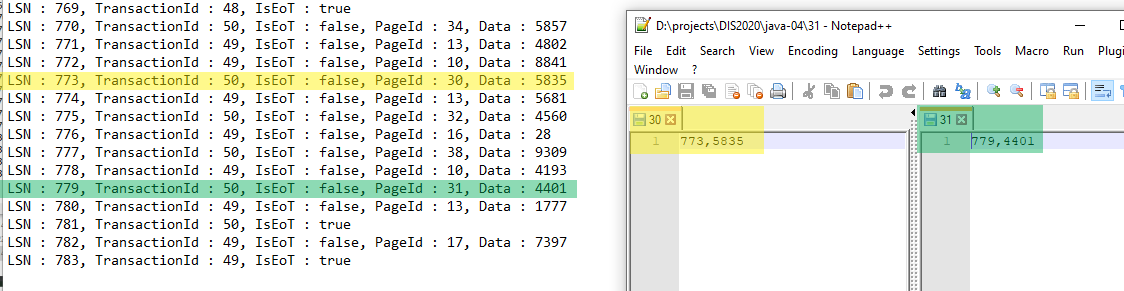
\includegraphics[width=\textwidth,height=\textheight,keepaspectratio]{c1_1.png}\\
	
	\textit{Deleting and modifying the pages:}\\
	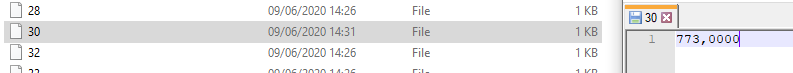
\includegraphics[width=\textwidth,height=\textheight,keepaspectratio]{c1_2.png}\\
	
	\textit{After recovery:}\\
	
\includegraphics[width=\textwidth,height=\textheight,keepaspectratio]{c1_3.png}\\
	
	The recovery failed for page \texttt{30} because the redo-recovery only checks for writes that satisfy \texttt{LSN(LS) > LSN(Page)}. We were wondering why \texttt{>} is not a \texttt{>=} because this small change would enable us to also recover from that error. For page \texttt{31} the recovery worked.
\end{itemize}
\begin{lstlisting}

\end{lstlisting}

\subsection*{c.2)}
\begin{lstlisting}

\end{lstlisting}

\subsection*{c.3)}
\begin{lstlisting}

\end{lstlisting}

\end{document}
